% !TeX program = xelatex
\documentclass[a4paper,10pt]{article}

% ============================================================================
% សន្លឹកកិច្ចការសិស្ស ស-ខ្មៅ (Student Worksheet - Grade 8 Lesson 1: 4 RAT_MUL)
% បរិបទ៖ គ្មានស្លាយ LCD និងគ្មានម៉ាស៊ីនគិតលេខ — សិស្សបំពេញផ្ទាល់លើសន្លឹកកិច្ចការ ២ ទំព័រ A4
% ============================================================================
\usepackage[a4paper, left=0.85cm, right=0.85cm, top=0.70cm, bottom=0.95cm, footskip=0.48cm]{geometry}
\usepackage{amsmath, amssymb}
\usepackage{unicode-math}
\usepackage{fontspec}
\usepackage{array, colortbl}
\usepackage[table]{xcolor}
\usepackage{enumitem}
\usepackage{pifont}
\usepackage{fancyhdr}
\usepackage{lastpage}
\usepackage{tikz}
\usepackage[most]{tcolorbox}
\usetikzlibrary{calc, arrows.meta, decorations.pathreplacing, positioning, babel}

\makeatletter
\let\@expl@@@mark@update@singlecol@structures@@\relax
\makeatother

\providecommand{\NGSFindFonts}{%
  \IfFileExists{C:/Windows/Fonts/cambria.ttc}{%
    \def\NGSSysPath{C:/Windows/Fonts/}%
    \def\NGSUserPath{C:/Users/KIT/AppData/Local/Microsoft/Windows/Fonts/}%
  }{%
    \IfFileExists{./fonts/KhmerOSsiemreap.ttf}{\def\NGSSysPath{./fonts/}\def\NGSUserPath{./fonts/}}{%
    \IfFileExists{../fonts/KhmerOSsiemreap.ttf}{\def\NGSSysPath{../fonts/}\def\NGSUserPath{../fonts/}}{%
    \IfFileExists{../../fonts/KhmerOSsiemreap.ttf}{\def\NGSSysPath{../../fonts/}\def\NGSUserPath{../../fonts/}}{%
    \IfFileExists{../../../fonts/KhmerOSsiemreap.ttf}{\def\NGSSysPath{../../../fonts/}\def\NGSUserPath{../../../fonts/}}{%
    \IfFileExists{../../../../fonts/KhmerOSsiemreap.ttf}{\def\NGSSysPath{../../../../fonts/}\def\NGSUserPath{../../../../fonts/}}{%
    \IfFileExists{../../../../../fonts/KhmerOSsiemreap.ttf}{\def\NGSSysPath{../../../../../fonts/}\def\NGSUserPath{../../../../../fonts/}}{%
    \IfFileExists{../../../../../../fonts/KhmerOSsiemreap.ttf}{\def\NGSSysPath{../../../../../../fonts/}\def\NGSUserPath{../../../../../../fonts/}}{%
      \def\NGSSysPath{../../../../../../../fonts/}\def\NGSUserPath{../../../../../../../fonts/}%
    }}}}}}}%
  }%
}
\NGSFindFonts

\setmathfont[Path={\NGSSysPath}, FontIndex=1, Scale=1.02]{cambria.ttc}
\defaultfontfeatures{Ligatures=TeX}

\setmainfont[
  Path={\NGSUserPath}, Extension=.ttf, Script=Khmer,
  BoldFont={KhmerOSsiemreap}, BoldFeatures={FakeBold=1.8},
  ItalicFont={KhmerOSsiemreap}, ItalicFeatures={FakeSlant=0.22}
]{KhmerOSsiemreap}

\newfontfamily\muol[Path={\NGSUserPath}, Extension=.ttf, Script=Khmer]{KhmerOSmuollight}
\newfontfamily\TimesEn[Path={\NGSSysPath}, Extension=.ttf, BoldFont={timesbd}, ItalicFont={timesi}]{times}

\XeTeXlinebreaklocale "km"
\XeTeXlinebreakskip = 0pt plus 1pt minus 0.1pt

\definecolor{panelgray}{gray}{0.93}
\definecolor{headgray}{gray}{0.85}

\pagestyle{fancy}
\fancyhf{}
\renewcommand{\headrulewidth}{0pt}
\fancyfoot[L]{\fontsize{7.5pt}{9.5pt}\selectfont អនុវិទ្យាល័យព្រះក្រសាំង \en{|} គណិតវិទ្យាថ្នាក់ទី៨ \en{|} មេរៀនទី១៖ ៤. ប្រមាណវិធីគុណ និងលក្ខណៈនៃវិធីគុណ (គ្រូ៖ ហុក ប៊ុនថែន)}
\fancyfoot[R]{\fontsize{7.8pt}{9.5pt}\selectfont ទំព័រ \en{\thepage/\pageref{LastPage}}}

\setlength{\parindent}{0pt}
\setlength{\parskip}{0pt}
\setlength{\tabcolsep}{3.8pt}

\newcommand{\en}[1]{{\TimesEn #1}}
\newcommand{\enbf}[1]{{\TimesEn\bfseries #1}}
\newcommand{\unit}[1]{\,\text{\en{#1}}}
\newcommand{\cnum}[1]{\mbox{\fontsize{10pt}{12pt}\selectfont\ding{\numexpr181+#1\relax}}}
\newcommand{\chkbox}{\tikz[baseline=-0.12ex]\draw[black, line width=0.8pt] (0,0) rectangle (0.24cm,0.24cm);}
\newcommand{\blank}[1][1.5cm]{\makebox[#1]{\dotfill}}
\newcommand{\secbar}[2]{%
  \begin{tcolorbox}[enhanced, sharp corners, colback=headgray, colframe=black, boxrule=0.9pt, boxsep=1pt, top=2pt, bottom=2pt, left=5pt, right=5pt, before skip=4pt, after skip=3pt]
    {\muol\fontsize{9.2pt}{13pt}\selectfont #1}\hfill{\fontsize{8pt}{11pt}\selectfont\textbf{#2}}
  \end{tcolorbox}%
}

\newcolumntype{L}[1]{>{\raggedright\arraybackslash}p{#1}}
\newcolumntype{C}[1]{>{\centering\arraybackslash}p{#1}}

\begin{document}
\fontsize{9.6pt}{14.4pt}\selectfont

% ============================================================================
% ទំព័រទី ១៖ E1 + E2 (POE 1 & POE 2) + E3 សំយោគបញ្ញត្តិ និងធនាគារហេតុផល
% ============================================================================
\begin{tcolorbox}[enhanced, sharp corners, colback=white, colframe=black, boxrule=1.0pt, boxsep=2pt, top=3pt, bottom=3pt, left=6pt, right=6pt]
  \begin{center}
    {\muol\fontsize{9.8pt}{14.8pt}\selectfont អនុវិទ្យាល័យព្រះក្រសាំង \enbf{--} សន្លឹកកិច្ចការសិស្ស \enbf{(}មេរៀនទី១៖ ៤\enbf{.} ប្រមាណវិធីគុណ និងលក្ខណៈនៃវិធីគុណ\enbf{)}}\\[3pt]
    {\fontsize{8.8pt}{12pt}\selectfont
    ឈ្មោះសិស្ស / ដៃគូ៖ \blank[5.2cm] \hspace{0.25cm}
    ថ្នាក់ទី៨៖ \blank[1.1cm] \hspace{0.25cm}
    ក្រុមទី៖ \blank[1.0cm] \hspace{0.25cm}
    កាលបរិច្ឆេទ៖ ២០/១១/២០២៦}
  \end{center}
\end{tcolorbox}

% --- E1 + E2 ---
\secbar{ផ្នែកទី១៖ បេសកកម្មទស្សន៍ទាយ \enbf{(E1)} និងការរុករកជាដៃគូ \enbf{(E2 -- POE 1 \& POE 2)}}{រយៈពេល ១៤ នាទី}

\begin{tcolorbox}[enhanced, sharp corners, colback=panelgray, colframe=black, boxrule=0.75pt, boxsep=1.5pt, top=2.5pt, bottom=2.5pt, left=5pt, right=5pt]
  \begin{minipage}{12.8cm}
    \textbf{បេសកកម្ម \en{E1} (គូសធីក \chkbox\ មុនពិសោធន៍)៖} សួនបន្លែការ៉េ $1\unit{m}^2$ គេយកបណ្ដោយ $\frac{2}{3}\unit{m}$ និងទទឹង $\frac{3}{4}\unit{m}$ ដាំស្ពៃ៖\\[2pt]
    (១) តើផ្ទៃដាំស្ពៃ $\frac{2}{3}\times\frac{3}{4}$ ធំជាង ឬតូចជាង $\frac{3}{4}\unit{m}^2$? \chkbox\ ធំជាង \quad \chkbox\ តូចជាង \quad \chkbox\ ស្មើគ្នា\\[2pt]
    (២) តើពេលគុណប្រភាគ ចាំបាច់តម្រូវភាគបែងរួមដូចវិធីបូកឬទេ? \chkbox\ ចាំបាច់ \quad \chkbox\ មិនចាំបាច់ \;\en{|}\; រាប់ក្រឡា៖ $\frac{\blank[0.6cm]}{12}=\blank[0.8cm]$
  \end{minipage}\hfill
  \begin{minipage}{4.7cm}
    \centering
    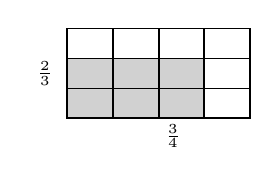
\begin{tikzpicture}[x=0.58cm, y=0.38cm, every node/.style={font=\scriptsize, text=black}]
      \foreach \c in {0,1,2} { \foreach \r in {0,1} { \fill[gray!36] (\c,\r) rectangle (\c+1,\r+1); } }
      \foreach \c in {0,...,3} { \foreach \r in {0,...,2} { \draw[black, line width=0.65pt] (\c,\r) rectangle (\c+1,\r+1); } }
      \node at (2.0,-0.58) {ទទឹង $\frac{3}{4}$};
      \node[anchor=east] at (-0.10,1.5) {$\frac{2}{3}$};
    \end{tikzpicture}
  \end{minipage}
\end{tcolorbox}

\vspace{4pt}
\textbf{ក. សកម្មភាពទី ១ (\en{POE 1})៖ រាប់សញ្ញាដក និងសម្រួលខ្វែងមុនគុណ (សៀវភៅពុម្ព ទំ.៨)}

{\renewcommand{\arraystretch}{1.58}
\begin{tabular}{|L{4.80cm}|L{8.80cm}|C{4.20cm}|}
  \hline
  \rowcolor{headgray}
  \textbf{លំហាត់គោល (ទំ.៨)} & \textbf{បំប្លែង សម្រួលខ្វែង និងរាប់សញ្ញាដកដោយដៃ} & \textbf{ផលគុណសម្រួលរួច} \\
  \hline
  ១. ក្រឡាផ្ទៃសួនបន្លែ (\en{E1})៖ $\dfrac{2}{3}\times\dfrac{3}{4}$ & មិនបាច់តម្រូវភាគបែងរួមទេ៖ $=\dfrac{2\times\blank[0.6cm]}{3\times\blank[0.6cm]} = \dfrac{6}{12}$ & $\blank[1.8cm]$ \\
  \hline
  ២. ឧទាហរណ៍ទី១៖ $\dfrac{3}{8}\times 3.8$ & $=\dfrac{3}{8}\times\dfrac{\blank[0.8cm]}{10} = \dfrac{3\times 19}{8\times \blank[0.7cm]}$ (សម្រួលនឹង $2$) & $\blank[1.8cm]$ \\
  \hline
  ៣. ឧទាហរណ៍ទី២៖ $\left(-\dfrac{2}{3}\right)\left(-\dfrac{7}{15}\right)$ & កត្តាដក $2$ តួ (គូ $\to \blank[0.5cm]$) $\implies \dfrac{2\times \blank[0.7cm]}{3\times 15}$ & $\blank[1.8cm]$ \\
  \hline
  ៤. គំរូ ឃ៖ $(-4)\left(-\dfrac{3}{5}\right)\left(\dfrac{5}{6}\right)\left(\dfrac{1}{2}\right)$ & កត្តាដក $2$ តួ $\implies +\dfrac{4\times 3\times 5\times 1}{1\times 5\times 6\times 2}$ (សម្រួល $5$ និង $12$!) & $\blank[1.8cm]$ \\
  \hline
\end{tabular}}

\vspace{4pt}
$\bullet$ \textbf{ពន្យល់ (\en{E})៖} ការសម្រួលខ្វែងមុនគុណ ធ្វើឱ្យលេខ \blank[1.8cm] ងាយគណនាដោយដៃ ដោយមិនបាច់គុណលេខធំ!

\vspace{4pt}
\textbf{ខ. សកម្មភាពទី ២ (\en{POE 2})៖ វែនតាឆ្លុះកត្តារួម \textbf{[គូសវង់កត្តារួម]} — លក្ខណៈបំបែក (លំហាត់គំរូ ក ទំ.៩)}

\begin{tcolorbox}[enhanced, sharp corners, colback=white, colframe=black, boxrule=0.7pt, boxsep=2pt, top=2.5pt, bottom=2.5pt, left=5pt, right=5pt]
  គណនា $\dfrac{7}{5}\cdot\dfrac{9}{4} + \dfrac{7}{5}\cdot\dfrac{11}{4}$ ដោយមិនគុណលេខធំដាច់ៗពីគ្នា៖ ចូរ \textbf{[គូសវង់កត្តារួម]} $\dfrac{7}{5}$ រួចទាញចេញក្រៅវង់ក្រចក៖\\[3pt]
  $\dfrac{7}{5}\cdot\dfrac{9}{4} + \dfrac{7}{5}\cdot\dfrac{11}{4} = \blank[1.0cm]\cdot\left(\dfrac{9}{4} + \dfrac{\blank[0.8cm]}{4}\right) = \dfrac{7}{5}\cdot\left(\dfrac{\blank[0.8cm]}{4}\right) = \dfrac{7}{5}\cdot\blank[0.8cm] = \blank[1.2cm]$ \quad (\textbf{ចំណាយពេលតែ ៥ វិនាទី!})
\end{tcolorbox}

% --- E3 ---
\secbar{ផ្នែកទី២៖ សំយោគបញ្ញត្តិ \enbf{(E3)} និងធនាគារហេតុផល \enbf{B\&W} \cnum{1}\enbf{--}\cnum{5}}{សៀវភៅពុម្ព ទំ.៨–៩}

\begin{tabular}{|L{9.20cm}|L{9.20cm}|}
  \hline
  \textbf{១. រូបមន្តគុណ ចំនួនច្រាស និងលក្ខណៈទាំង ៦ (ទំ.៨–៩)៖}\par\vspace{2.5pt}
  $\bullet$ \textbf{ជាទូទៅ៖} $\dfrac{a}{b}\cdot\dfrac{c}{d} = \dfrac{\blank[1.1cm]}{\blank[1.1cm]}$ ($b,d\neq 0$)\par\vspace{2.5pt}
  $\bullet$ \textbf{ក្បួនសញ្ញា៖} សញ្ញាដូចគ្នា $\to \blank[0.6cm]$ \;;\; សញ្ញាផ្ទុយគ្នា $\to \blank[0.6cm]$\par\vspace{2.5pt}
  $\bullet$ \textbf{ចំនួនច្រាស (លក្ខណៈទី៥)៖} $\dfrac{a}{b}\cdot\dfrac{\blank[0.7cm]}{\blank[0.7cm]} = 1$ ($a,b\neq 0$)\par\vspace{2.5pt}
  $\bullet$ \textbf{លក្ខណៈបំបែក (ទី៦)៖} $\dfrac{a}{b}\left(\dfrac{c}{d}\pm\dfrac{e}{f}\right) = \dfrac{a}{b}\cdot\dfrac{c}{d} \pm \blank[1.5cm]$
  &
  \textbf{២. ធនាគារហេតុផល \en{B\&W} (\cnum{1}--\cnum{5})៖}\par\vspace{2.5pt}
  \cnum{1} យកភាគយកគុណភាគយក និងភាគបែងគុណភាគបែង ($\frac{ac}{bd}$) ។\par\vspace{2.5pt}
  \cnum{2} រាប់ចំនួនកត្តាដកជាមុន៖ ចំនួនគូ $\to +$ ; ចំនួនសេស $\to -$ ។\par\vspace{2.5pt}
  \cnum{3} បំប្លែងចំនួនចម្រុះ/ទសភាគជាប្រភាគសិន រួចសម្រួលខ្វែងមុនគុណ ។\par\vspace{2.5pt}
  \cnum{4} ចំនួនច្រាសនៃ $\frac{a}{b}$ គឺ $\frac{b}{a}$ (រក្សាសញ្ញាដដែល; $0$ គ្មានច្រាសទេ) ។\par\vspace{2.5pt}
  \cnum{5} លក្ខណៈបំបែក/ផ្គុំ៖ គូសវង់ទាញកត្តារួម ឬផ្គុំគូសម្រួលដាច់ ។ \\
  \hline
\end{tabular}

\vspace{4pt}
\begin{tcolorbox}[enhanced, sharp corners, colback=panelgray, colframe=black, boxrule=0.65pt, boxsep=1.5pt, top=2pt, bottom=2pt, left=5pt, right=5pt]
  \textbf{ប្រយ័ត្នអន្ទាក់៖} (១) ចំនួនច្រាសនៃ $-\frac{3}{5}$ គឺ $-\frac{5}{3}$ (\textbf{រក្សាសញ្ញាដក} ព្រោះផលគុណស្មើ $+1$)! \quad (២) $5\frac{3}{4}\times\frac{12}{125}$ ត្រូវបំប្លែង $5\frac{3}{4}=\frac{23}{4}$ សិន!
\end{tcolorbox}

\vspace{4pt}
\textbf{៣. លំហាត់ត្រួតពិនិត្យរហ័ស៖ គណនាផលគុណ និងរកចំនួនច្រាសដោយដៃ}

\vspace{2.5pt}
{\renewcommand{\arraystretch}{1.64}
\begin{tabular}{|C{4.40cm}|C{4.40cm}|C{4.40cm}|C{4.40cm}|}
  \hline
  \rowcolor{panelgray}
  $\frac{3}{5}\times\frac{5}{9} = \blank[1.1cm]$ & $\left(-\frac{3}{4}\right)\left(-\frac{8}{9}\right) = \blank[1.0cm]$ & ច្រាសនៃ $\frac{4}{7}$ គឺ $\blank[1.0cm]$ & $0.25\times 16 = \blank[1.0cm]$ \\
  \hline
  $\left(-\frac{2}{7}\right)\times\frac{14}{3} = \blank[1.0cm]$ & $\frac{5}{8}\times 0 = \blank[1.1cm]$ & ច្រាសនៃ $-\frac{3}{5}$ គឺ $\blank[1.0cm]$ & $0.75\times 12 = \blank[1.0cm]$ \\
  \hline
  $\left(-\frac{6}{11}\right)\left(-\frac{11}{6}\right) = \blank[0.9cm]$ & $(-1)(-2)\left(-\frac{1}{2}\right) = \blank[0.9cm]$ & ច្រាសនៃ $-4$ គឺ $\blank[1.0cm]$ & $1\frac{1}{2}\times\frac{2}{3} = \blank[1.0cm]$ \\
  \hline
  $\frac{4}{9}\times\frac{3}{8} = \blank[1.1cm]$ & $\left(-\frac{5}{6}\right)\times 1 = \blank[1.0cm]$ & ផ្ទុយនៃ $-\frac{3}{5}$ គឺ $\blank[1.0cm]$ & $(-0.5)(-0.2) = \blank[0.9cm]$ \\
  \hline
\end{tabular}}

\newpage

% ============================================================================
% ទំព័រទី ២៖ E4 លំហាត់គំរូ + E5 ប្រតិបត្តិ & វិនិច្ឆ័យ A-D + Exit + កិច្ចការផ្ទះ
% ============================================================================
\secbar{ផ្នែកទី៣៖ ពង្រីកចំណេះដឹងលើទសភាគ និងលក្ខណៈផ្គុំ\enbf{-}បំបែក \enbf{(E4 --} ទំ\enbf{.}៨ និងទំ\enbf{.}៩\enbf{)}}{រយៈពេល ១០ នាទី}

\textbf{លំហាត់ពង្រីកចំណេះដឹង៖} ចូរបំពេញជំហានគណនាខាងក្រោមដោយដៃ ព្រមទាំងបញ្ជាក់លេខហេតុផល \cnum{1}--\cnum{5}៖

{\renewcommand{\arraystretch}{1.52}
\begin{tabular}{|L{4.70cm}|L{9.10cm}|C{4.00cm}|}
  \hline
  \rowcolor{headgray}
  \textbf{លំហាត់គំរូ (ទំ.៨ និង ៩)} & \textbf{ដំណើរការគណនាដោយដៃតាមលក្ខណៈនៃវិធីគុណ} & \textbf{ចម្លើយ និងហេតុផល} \\
  \hline
  \textbf{១. គំរូ ក, ខ (ទំ.៨)}\par\vspace{2pt}ក) $0.25\times 48$ \;;\; ខ) $245.4\times 5.3$ & ក) $=\dfrac{1}{\blank[0.6cm]}\times 48 = \blank[0.9cm]$ \;\en{|}\; ខ) គុណដូចចំនួនគត់ រួចកាត់ក្បៀស $2$ ខ្ទង់ & ក)$=\blank[0.9cm]$\par\vspace{1.5pt}ខ)$=\blank[1.2cm]$ \\
  \hline
  \textbf{២. គំរូ គ (ទំ.៨)}\par\vspace{2pt}$(-3.2)(7.4)(-0.1)(-0.5)$ & កត្តាដក $3$ តួ (សេស $\to \blank[0.5cm]$)៖ $[(-3.2)(-0.5)][(7.4)(-0.1)] = (1.6)(\blank[1.0cm])$ & $=\blank[1.4cm]$ (\cnum{2}) \\
  \hline
  \textbf{៣. គំរូ ខ (ទំ.៩ — បំបែក)}\par\vspace{2pt}$\dfrac{4}{5}\cdot\dfrac{9}{4} - \dfrac{7}{8}\cdot\dfrac{4}{5}$ & ទាញកត្តារួម $\dfrac{4}{5}$៖ $=\dfrac{4}{5}\cdot\left(\dfrac{9}{4} - \dfrac{7}{8}\right) = \dfrac{4}{5}\cdot\left(\dfrac{18 - \blank[0.7cm]}{8}\right)$ & $=\blank[1.4cm]$ (\cnum{5}) \\
  \hline
  \textbf{៤. គំរូ គ (ទំ.៩ — ផ្គុំ)}\par\vspace{2pt}$\dfrac{-3}{5}\left(\dfrac{7}{8}\cdot\dfrac{10}{-3}\right)$ & ផ្គុំគូសម្រួលដាច់៖ $=\dfrac{7}{8}\cdot\left(\dfrac{-3}{5}\cdot\dfrac{10}{-3}\right) = \dfrac{7}{8}\cdot\blank[0.8cm]$ & $=\blank[1.4cm]$ (\cnum{5}, \cnum{3}) \\
  \hline
\end{tabular}}

\vspace{4pt}
$\bullet$ \textbf{សំណួរឆ្លុះបញ្ចាំង \en{(EIA Looking-Back)}៖} តើ\textbf{ចំនួនផ្ទុយ} និង\textbf{ចំនួនច្រាស}នៃ $-\dfrac{3}{5}$ ខុសគ្នាដូចម្ដេច?\\
ចម្លើយ៖ ចំនួនផ្ទុយគឺ \blank[1.2cm] (ផលបូកស្មើ $0$) រីឯចំនួនច្រាសគឺ \blank[1.2cm] (ផលគុណស្មើ $+1$, \cnum{4}) ។

% --- E5 ---
\secbar{ផ្នែកទី៤៖ វាយតម្លៃលទ្ធផលសិក្សា \enbf{(E5 --} ប្រតិបត្តិ ទំ\enbf{.}៩ \enbf{+} វិនិច្ឆ័យ \enbf{A--D +} សំបុត្រចេញ\enbf{)}}{រយៈពេល ១០ នាទី}

\textbf{ក. លំហាត់ប្រតិបត្តិ (សៀវភៅពុម្ព ទំ.៩ ផ្នែកលើ និងផ្នែកក្រោម — ធ្វើជាដៃគូ \en{Pause-Review})៖}

{\renewcommand{\arraystretch}{1.48}
\begin{tabular}{|L{8.90cm}|L{8.90cm}|}
  \hline
  \textbf{១) ប្រតិបត្តិផ្នែកលើ (ទំ.៩)៖}\par\vspace{2.5pt}
  $\bullet$ \textbf{ក)} $0.75\times\dfrac{13}{125} = \dfrac{\blank[0.6cm]}{4}\times\dfrac{13}{125} = \blank[1.4cm]$\par\vspace{2.5pt}
  $\bullet$ \textbf{ខ)} $5\dfrac{3}{4}\times\dfrac{12}{125} = \dfrac{\blank[0.7cm]}{4}\times\dfrac{12}{125} = \blank[1.4cm]$\par\vspace{2.5pt}
  $\bullet$ \textbf{គ)} $\left(-\dfrac{1}{3}\right)\left(\dfrac{3}{5}\right)(0.5)(0.2) = \left(-\dfrac{1}{5}\right)(\blank[0.8cm]) = \blank[1.2cm]$
  &
  \textbf{២) ប្រតិបត្តិផ្នែកក្រោម (ទំ.៩ — ប្រើលក្ខណៈគុណ)៖}\par\vspace{2.5pt}
  $\bullet$ \textbf{ក)} $\dfrac{9}{5}\cdot\dfrac{3}{4}-\dfrac{9}{5}\cdot\dfrac{11}{4} = \dfrac{9}{5}\left(\dfrac{3-11}{4}\right) = \blank[1.4cm]$\par\vspace{2.5pt}
  $\bullet$ \textbf{ខ)} $\dfrac{2}{3}\cdot\left(\dfrac{3}{4}-\dfrac{7}{8}\right) = \dfrac{2}{3}\cdot\left(\dfrac{\blank[0.8cm]}{8}\right) = \blank[1.4cm]$\par\vspace{2.5pt}
  $\bullet$ \textbf{គ)} $\left(-\dfrac{3}{7}\cdot\dfrac{10}{12}\right)\cdot\dfrac{6}{10} = \blank[1.4cm]$ \;\en{|}\; \textbf{បិទ \en{E1}៖} $\blank[1.0cm]\unit{m}^2$ \\
  \hline
\end{tabular}}

\vspace{5pt}
\textbf{ខ. គូសវង់ជុំវិញជម្រើសត្រឹមត្រូវតែ ១ គត់ ក្នុងចំណោម \en{A, B, C, D} រួចសរសេរលេខហេតុផល \cnum{1}--\cnum{5}៖}

{\renewcommand{\arraystretch}{1.75}
\begin{tabular}{|L{8.90cm}|L{8.90cm}|}
  \hline
  \rule[-9pt]{0pt}{24pt}\textbf{ជម្រើស \en{A}៖} $5\dfrac{3}{4}\times\dfrac{12}{125} = 5\dfrac{36}{500}$ &
  \textbf{ជម្រើស \en{B}៖} ចំនួនច្រាសនៃ $-\dfrac{4}{7}$ គឺ $+\dfrac{7}{4}$ \\
  \hline
  \rule[-9pt]{0pt}{24pt}\textbf{ជម្រើស \en{C}៖} $\dfrac{9}{5}\cdot\dfrac{3}{4}-\dfrac{9}{5}\cdot\dfrac{11}{4} = \dfrac{9}{5}(-2) = -\dfrac{18}{5}$ &
  \textbf{ជម្រើស \en{D}៖} $(-3.2)(7.4)(-0.1)(-0.5) = +1.184$ \\
  \hline
\end{tabular}}

\vspace{4pt}
\begin{tcolorbox}[enhanced, sharp corners, colback=panelgray, colframe=black, boxrule=0.75pt, boxsep=1.5pt, top=2.5pt, bottom=2.5pt, left=5pt, right=5pt]
  \textbf{សំបុត្រចេញពីថ្នាក់ (\en{Exit Ticket} — ៦០ វិនាទី)៖} គូសវង់កត្តារួម រួចគណនា និងរកចំនួនច្រាស៖\\
  (១) $\dfrac{5}{6}\cdot\dfrac{7}{10} + \dfrac{5}{6}\cdot\dfrac{13}{10} = \blank[0.9cm]\cdot\left(\dfrac{7+13}{10}\right) = \blank[1.2cm]$ \quad \en{|} \quad (២) ចំនួនច្រាសនៃ $-\dfrac{5}{6}$ គឺ \blank[1.1cm] (ហេតុផល \blank[0.9cm])
\end{tcolorbox}

% --- កិច្ចការផ្ទះ ---
\secbar{ផ្នែកទី៥៖ កិច្ចការផ្ទះ \enbf{(}សៀវភៅពុម្ព ទំ\enbf{.}១២ \enbf{\#10)} និងបណ្ដាំផ្ញើ}{ធ្វើក្នុងសៀវភៅកិច្ចការផ្ទះ}
$\bullet$ \textbf{លំហាត់ ១ (ទំ.១២ \#10ក,ខ)៖} គណនា៖ ក) $-\dfrac{4}{5}\cdot\left(\dfrac{11}{17}\cdot\dfrac{10}{16}\right)$ \qquad ខ) $-\left(\dfrac{11}{13}\cdot\dfrac{17}{16}\right)\cdot\dfrac{26}{51}$\\
$\bullet$ \textbf{លំហាត់ ២ (ទំ.១២ \#10ឃ,ច)៖} ក) $-\dfrac{11}{8}\cdot\dfrac{21}{22}+\dfrac{17}{16}\cdot\dfrac{21}{22}$ \quad ខ) $\left(-\dfrac{11}{21}\right)\cdot\dfrac{3}{7}+\left(\dfrac{-3}{7}\right)\cdot\left(-\dfrac{11}{21}\right)$ \;\en{|}\; \textbf{អានមុន៖} ចំណុច \textbf{៥. ប្រមាណវិធីចែក} (ទំ.១០) ។

\end{document}
